\section{Performance} \label{sec:perform}

The Start Counter was installed in Hall-D just prior to the Fall 2014 \gx{} commissioning run.  It was not until the Spring 2015 commissioning run that enough statistics were obtained with an $\mathrm{LH_{2}}$ target to perform reliable calibrations.  With the aforementioned data set the procedures to calibrate the detector, as discussed in Sec.~\ref{sec:calib}, and measure it's performance were developed and deployed.

As was discussed in previous sections, the geometry of the ST nose section results in an increase of the light output as the scintillation source moves towards the downstream end.  While investigating FADC250 data under nominal beam conditions, this phenomenon was immediately observed through both the pulse amplitude and pulse integral data. Figure~\ref{fig:pippvszint} illustrates that, similar to the bench measurements, the light output increases exponentially as the scintillation source moves towards the downstream end.
	\begin{figure}[!htb]
		\centering
		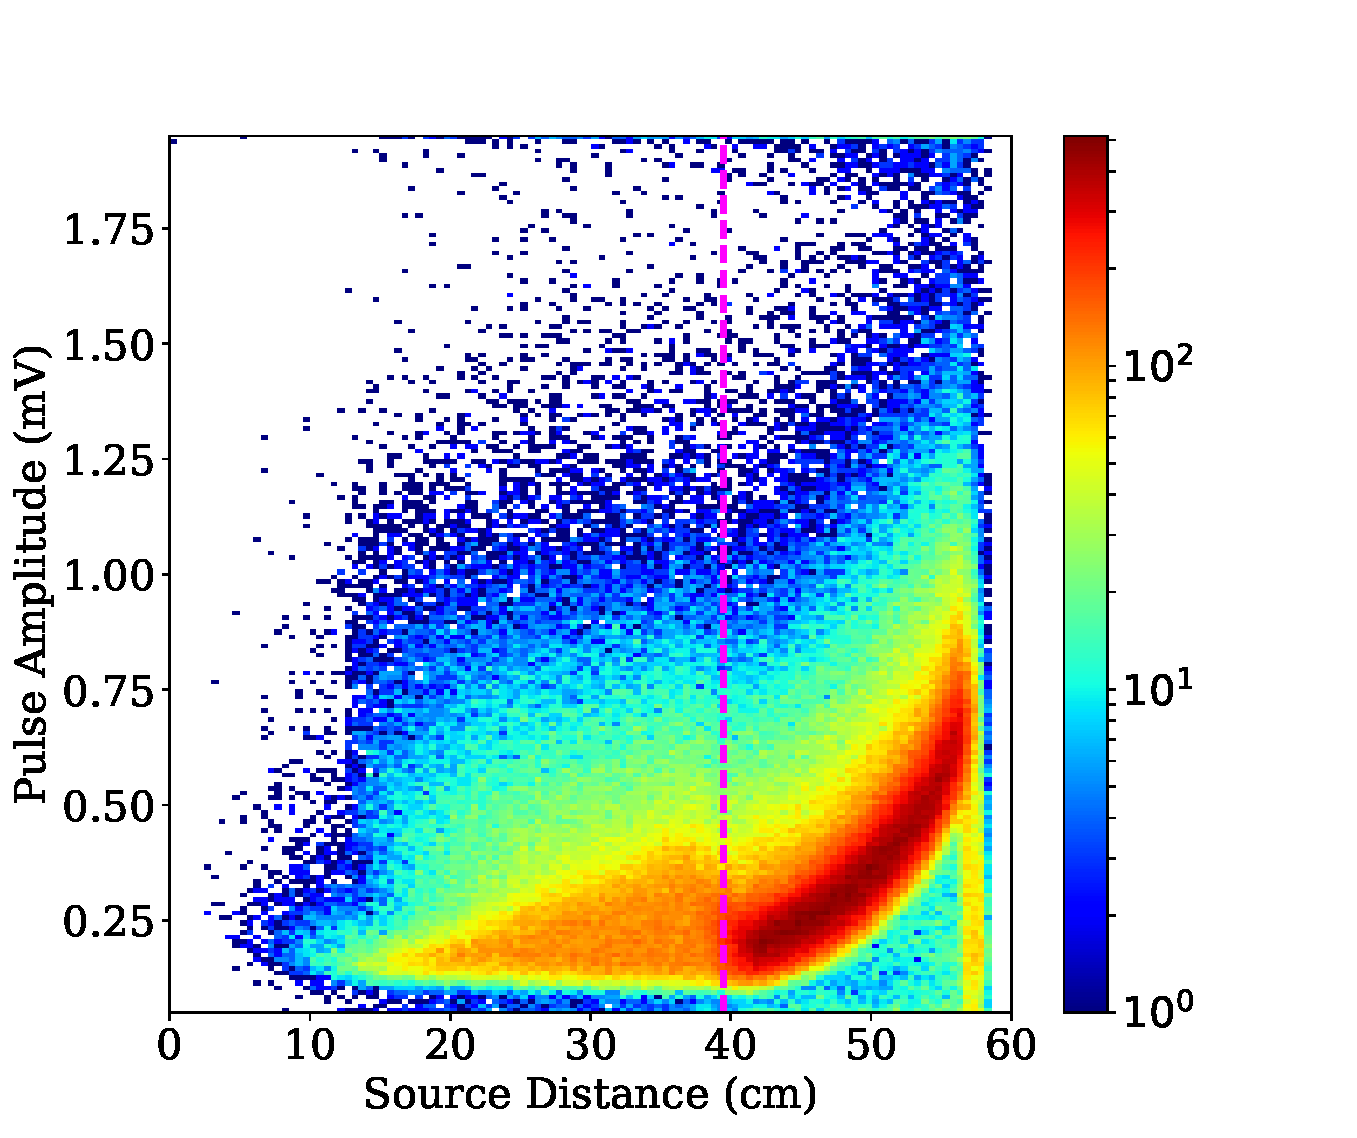
\includegraphics[width=1.0\columnwidth]{performance/figs/PPZ}
		\caption{Typical FADC250 pulse amplitude spectrum versus the $z$-component of charged tracks intersecting the ST for an individual ST sector. The vertical lines  indicate (from left to right) the end of the straight section, and the start of the tapered nose section respectively.}
		\label{fig:pippvszint}
	\end{figure}
This feature of the ST geometry is quite advantageous since the majority of the charged tracks produced under the nominal \gx{} beam conditions intersect the ST in the nose region and therefore have the largest light amount of light collected by the SiPM's at the upstream end.

Once the proper attenuation corrections discussed in Sec.~\ref{sec:calib_ac} were applied to the data, the PID capabilities of the ST were improved.  Figure ~\ref{fig:dEdx_vs_p_corr} illustrates the PID capability of charged tracks intersecting the ST.  
	\begin{figure}[!htb]
		\centering
		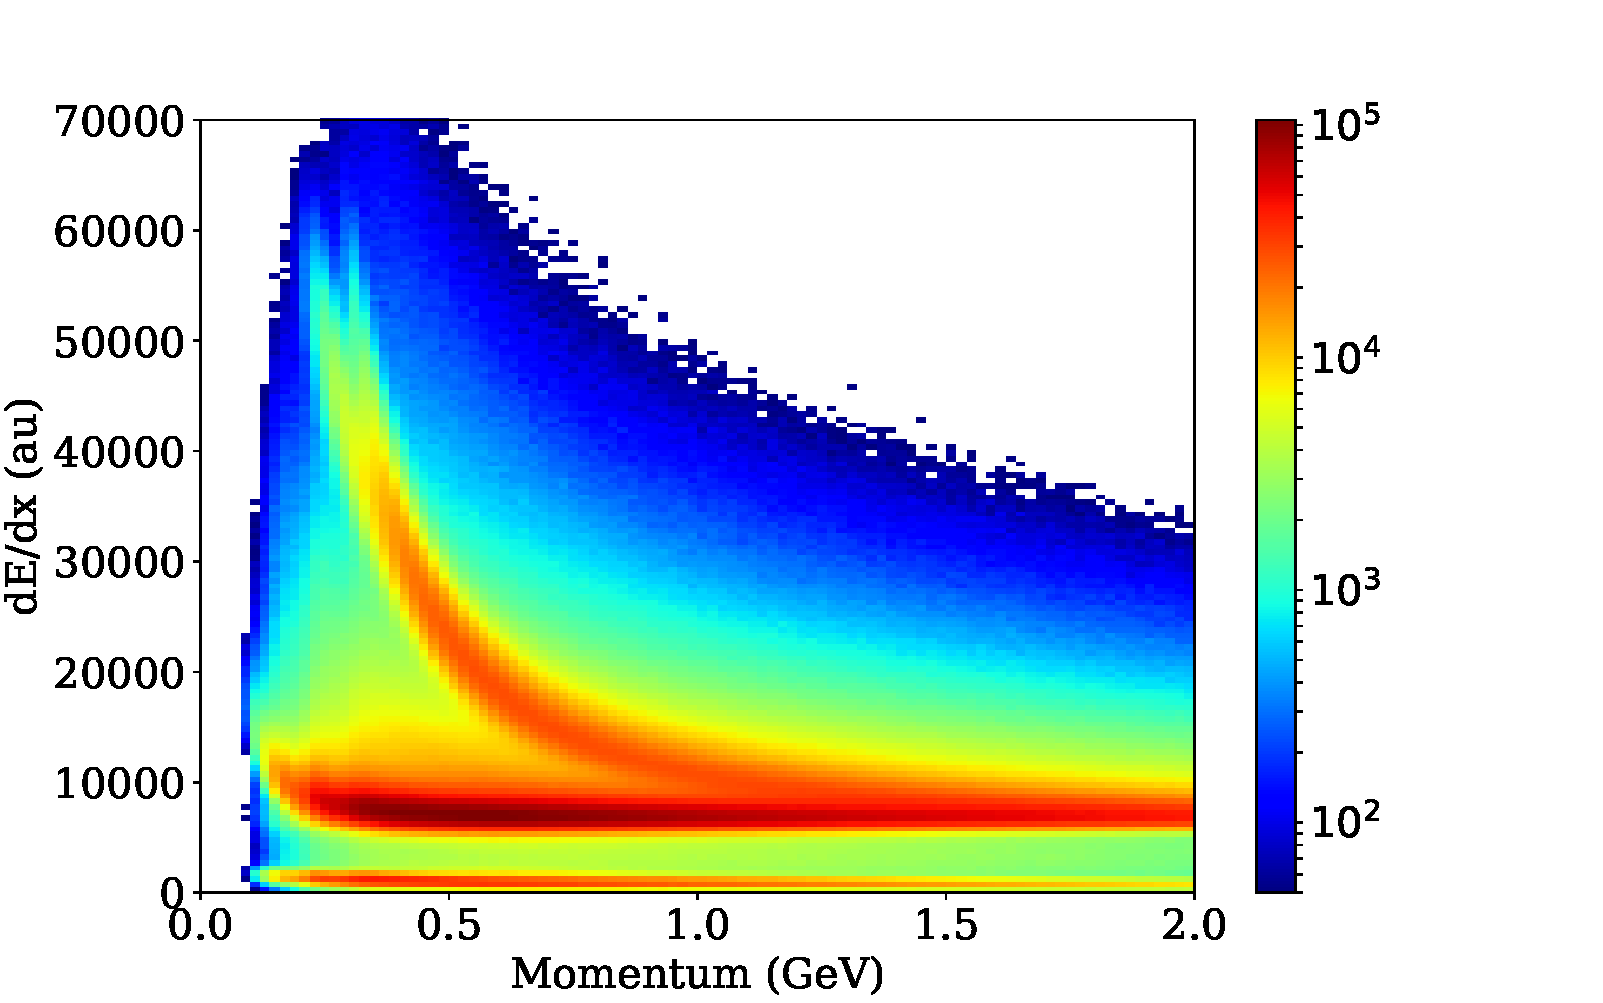
\includegraphics[width=1.0\columnwidth]{performance/figs/Att_corr}
		\caption{Corrected $dE/dx\ vs.\ p$ distribution for tracks matched to the Start Counter.  The ``banana band'' corresponds to protons while the horizontal band corresponds to electrons, pions, and kaons.  It is clear that pion/proton separation is achievable for tracks with $p < 0.9\ \mathrm{GeV/c}$.}
		\label{fig:dEdx_vs_p_corr}
	\end{figure}  
The reliable separation of protons and other hadrons occurs for charged tracks with $p < 0.9\ \mathrm{GeV/c}$ which is a factor 1.5 improvement relative to the uncalibrated data.  The PID capabilities of the ST are particularly advantageous for successfully identifying low momentum and backwards going protons which do not propagate into the central drift chamber surrounding the ST.

After the time-walk and propagation time corrections discussed in Sec.~\ref{sec:calib_tw} \& \ref{sec:calib_ptc} were complete, it was then possible to utilize the ST to measure times associated with charged track vertices for tracks matched to it.  The vertex time (Eq.~\ref{eq:st_vertex_time})  is defined to be the time when a polarized Bremsstrahlung photon interacted with the $\mathrm{LH_{2}}$ target and produced a charged track.  Measuring the ST vertex time relative to the beam bunch vertex time provided by the accelerator is the most robust way to determine the ST ability to successfully identify the beam buckets associated with a particular event.  An identical charged track selection process, as outlined in Sec.~\ref{sec:calib_ptc}, was utilized so that the time resolution of tracks matched to the ST could be measured.  

The resulting time difference distribution is seen in Fig. \ref{fig:st_time_res}.
	\begin{figure}[!htb]
		\centering
		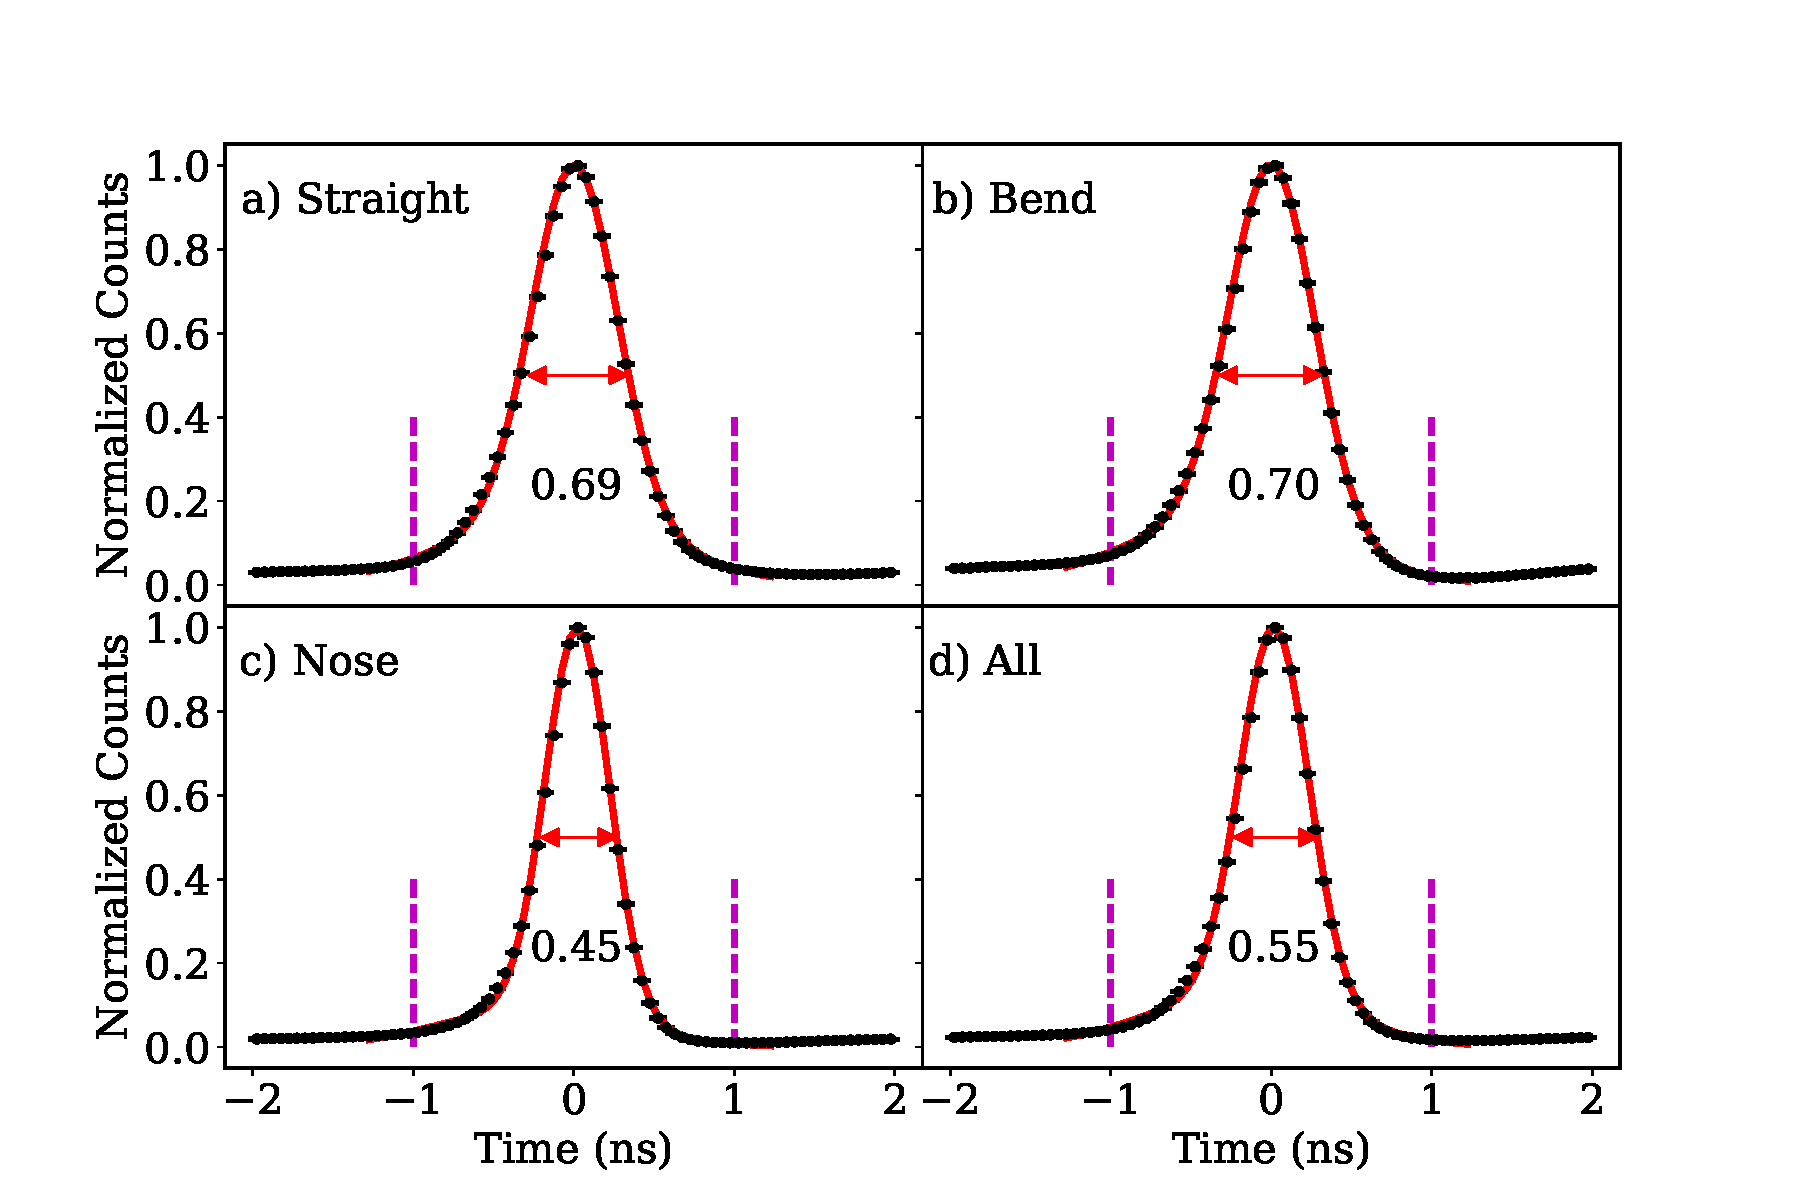
\includegraphics[width=1.08\linewidth]{performance/figs/TR_2gaussian}
		\caption{Start Counter  resolution  histograms and their full width half maxima (FWHM) values in ns.  The x-axis is the time difference between $T^{ST}_{vertex}$ and $T^{BB}_{vertex}$. The vertical lines indicate the cuts necessary to identify a beam bunch, a) The resolution in the straight section. b) The resolution in the bend section. c) The resolution in the nose. d) The resolution along the entire length of the paddle. }
		\label{fig:st_time_res}
	\end{figure}
% EP This plot is not needed, the results should be summarized in a table.
%	\begin{figure}[!htb]
%		\centering
%		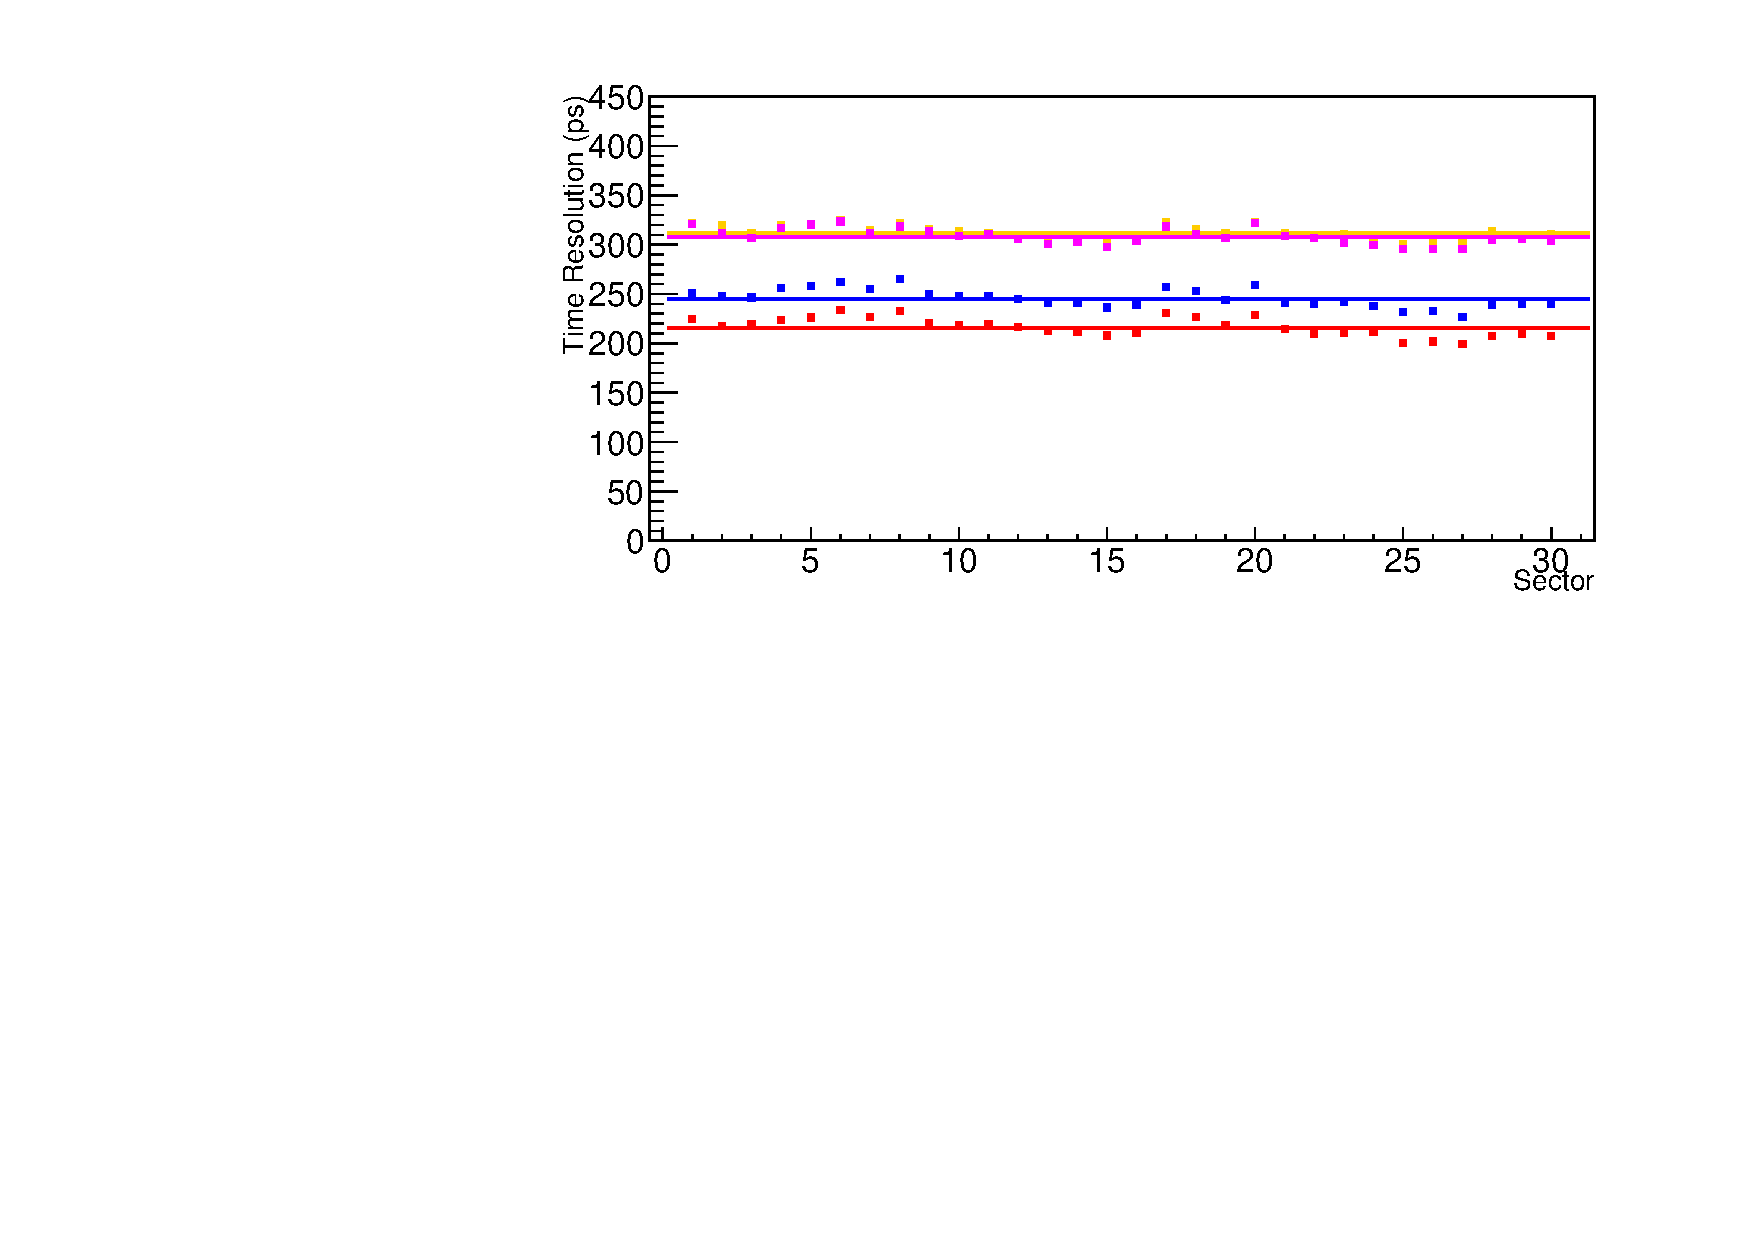
\includegraphics[width=1.08\columnwidth]{performance/figs/TR_All}
%		\caption{ST time resolutions as a function of sector number (Blue line). Orange and magenta lines are the average time resolution for the straight and bend sections respectively. The nose section resolution is greatly enhanced due to the exponential increase in light output (red).}
%		\label{fig:timeresallinset}
%	\end{figure}	
Fitting a single gaussian to the top $\approx 70\%$ percent of the measured distribution function can be used to characterize the overall time resolution quality. However in order to fit the measured distributions within a window of $\pm$ 1 ns a sum of two gaussian was necessary. The time resolution then can be characterized by its full width half maximum (FWHM) and by the fraction of events lying within a $\pm$ 1 ns boundary as this is typically the cut applied to identify a beam bunch.  

%The aforementioned fits were carried out for each of the ST sectors with $\sigma$ and its associated error being calculated.  Then a weighted average of the 30 $\sigma$'s were calculated so that the ST could have its time resolution characterized in its entirety.  

The aforementioned fits were carried out for the three individual geometrical sections and all 30 paddles and  Table~\ref{tab:time_res_section} details the results.
	\begin{table}[htbp]
		\centering
		\begin{tabular}{|c|c|c|c|c|}
			\hline  \textbf{Section} & $\mathbf{All}$ & $\mathbf{straight}$ & $\mathbf{Bend}$ & $\mathbf{Nose}$ \\ 
			\hline $\mathbf{\sigma_{FWHM}}$ & 550 ps & 690 ps & 700 ps & 450 ps \\
			\hline $\mathbf{Fraction}$ & 93\% & 92\% & 91\% &  94\% \\ 
			\hline 
		\end{tabular}
		\caption{Average time resolutions (FWHM) and event fractions within a $\pm$ 1~ns window for all 30 ST sectors by independent geometrical regions.}
		\label{tab:time_res_section}
	\end{table}

The ST exhibited uniformity in time resolution among all sectors of the ST. The high overall event fraction and good time resolution in the data for all sections combined is due to the fact that the majority of events intersect the ST in the nose section. 
%The data also indicates that the average time resolution of 245~ps is well below the design resolution of 350~ps.  
It is clear from Table~\ref{tab:time_res_section} that what is observed is that measurements made with beam data exhibit the same phenomenon of substantial improvement in light collection, and thus time resolution, as light is produced further downstream in the nose region.

When these time resolution measurements were conducted with data collected in Spring 2017, approximately 3 years had elapsed since the paddles were first tested on the bench at FIU.  Prior experience with degrading scintillators indicates that degradation in time resolution will be visible in a matter of weeks.  However, after 3 years no degradation has been observed and the ST is still performing well below design resolution.